%\renewcommand{\theequation}{\theenumi}
%\begin{enumerate}[label=\thesection.\arabic*.,ref=\thesection.\theenumi]
%\numberwithin{equation}{enumi}
Let
\begin{align}
\vec{A}=\myvec{-4\\5}
\vec{B}=\myvec{0\\7}
\vec{C}=\myvec{5\\-5}
\vec{D}=\myvec{-4\\-2}
\end{align}
Quadrilateral ABCD is drawn by joining its vertices $\vec{A}$ and $\vec{B}$,$\vec{B}$ and $\vec{C}$, $\vec{C}$ and $\vec{D}$, $\vec{D}$ and $\vec{A}$.
 The  following Python code generates Fig. \ref{fig:2.2.3_quad_py}
%
\begin{lstlisting}
codes/quad/quad.py
\end{lstlisting}
\begin{figure}[!ht]
\centering
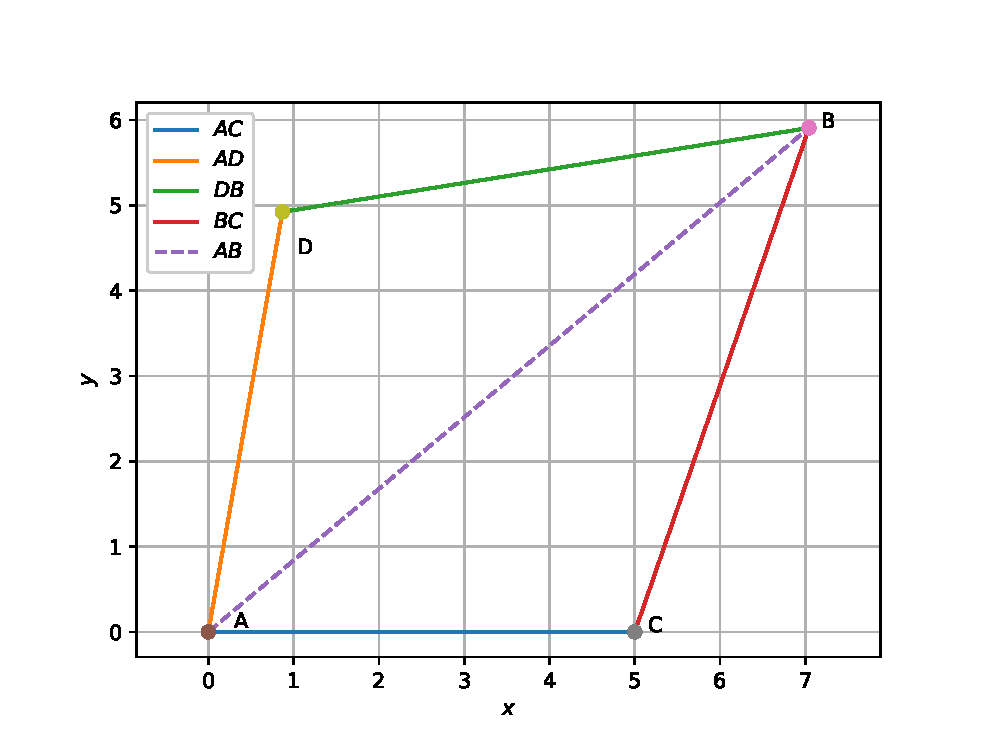
\includegraphics[width=\columnwidth]{./solutions/3/codes/quad/pyfigs/quad.eps}
\caption{Quadrilateral ABCD}
\label{fig:2.2.3_quad_py}
\end{figure}

 From Figure \ref{fig:2.2.3_quad_py} Area of the Quadrilateral ABCD can be given as
\begin{align}
Ar\brak{\triangle ABC} + Ar\brak{\triangle BCD}
\\
\frac{1}{2} \norm{\brak{\vec{A}-\vec{B}}\times \brak{\vec{A}-\vec{D}}} + \frac{1}{2} \norm{{\brak{\vec{C}-\vec{B}}} \times{\brak{\vec{C}-\vec{D}}}}
\label{eq:2.2.3_quad_area}
\end{align}
For two vectors $\vec{a} = \myvec{a_1\\a_2}$ and $\vec{b} = \myvec{b_1\\b_2}$
\begin{align}
\label{eq:2.2.3_cross_product}
\norm{\vec{a} \times \vec{b}} = |a_1 b_2- a_2 b_1|
\\
\vec{A}-\vec{B} = \myvec{-4\\-2}
\\
\vec{A}-\vec{D} = \myvec{0\\7}
\\
\vec{C}-\vec{B} = \myvec{5\\-12}
\\
\vec{C}-\vec{D} = \myvec{9\\-3}
\end{align}
Using \eqref{eq:2.2.3_cross_product}
\begin{align}
\frac{1}{2} \norm{\brak{\vec{A}-\vec{B}}\times \brak{\vec{A}-\vec{D}}} &= \frac{1}{2} |\brak{-28}| 
\\
&=14
\\
\frac{1}{2} \norm{\brak{\vec{C}-\vec{B}} \times \brak{\vec{C}-\vec{D}}} &= \frac{1}{2} |\brak{-15+108}|
\\
&=46.5
\end{align}
Substituting the above values in equation \eqref{eq:2.2.3_quad_area},We get
\begin{align}
Area = 14 + 46.5 = 60.5 sq.units
\end{align}
%\end{enumerate}
